\begin{comment}
\subsection{Self-organizing numbers}
\label{sec:sonums}

The design of floating-point numbers in the 1970s and 1980s was motivated to meet several criteria: (i) hardware-friendly, i.e. the number format was designed to map easily from existing arithmetic circuits into bits; (ii) multi-purpose, i.e. initially declared as format for \emph{scientific computations} it was supposed to be able to represent very large numbers $O(10^{-100})$ to $O(10^{-300})$ as well as very tiny numbers $O(10^{-100})$ to $O(10^{-300})$ with the same precision, to allow the use in many different fields of science (iii) error analysis-friendly, i.e. especially Float64 was designed to allow for very precise calculations, such that most scientists would not need to perform a numerical error analysis.

In the following we will relax these criteria and seek to find a number format that has the lowest rounding errors for a given application. We thereby ignore any hardware limitations, and create this number format purely on the basis of a software emulator. In fact, we end up designing it based on look-up tables. Arithmetic operations are with look-up tables not functions that calculate the result based on the inputs, but return the result from an array where the inputs determine the indices. This is in general only feasible for a small set of different inputs, as the underlying arrays have to be stored in memory. Look-up tables for 16-bit arithmetic, as considered here, are of a size of several GB which is unfeasible for current computing hardware. Look-up tables therefore are stored in RAM whereas a storage in much smaller low-level caches is necessary for speed. Every additional bit quadruples the size, such that look-up tables are only attractive for very low precision number formats or can be used for software emulators for up to 16 bit. We also do not aim to create a multi-purpose number format, but conversely a number format that is flexible enough to accommodate the precision requirements of a given algorithm as good as possible.

Motivated by the decimal precision analysed in the previous sections for floats and posits, the new number format is supposed to represent numbers in a given application with most precision for the numbers that occur most frequently and with no bitpatterns for numbers that never occur. Consequently, this number format is supposed have bitpatterns that occur equally frequent. This concept aligns with maximising entropy, which will be discussed in the next section. In analogy to the unsupervised learning of self-organizing maps, which are mostly used in two or more dimensions, we call the new number format self-organizing numbers, or \emph{sonums} in short. Note that the self-organization is here carried out on the real number axis, i.e. in one dimension.

We will make use of ideas introduced by the posit framework as introduced in section \ref{sec:posits} as most redundant bitpatterns that occur in floats ($\pm0$,$\pm\infty$, and a very large share of bitpatterns for NaNs, see Table \ref{tab:formats}) are removed for posits and only 2 bitpatterns for zero and NaR are retained as exceptions. The sonum circle is therefore designed in analogy to the posit circle (Fig. \ref{fig:circle}), but will be populated differently except for zero and NaR, which are mapped to identical bitpatterns for both formats. As illustrated in Fig. \ref{fig:sonum_circle} sonums retain the symmetry with respect to zero, such that there is a reversible map (the two's complement, \cite{Choo2003}) between a number and its negation. However, sonums do not have a symmetry with respect to the multiplicative inverse as posits or floats have (note that for posits or floats this symmetry is only perfect when the significand is zero, otherwise rounding is applied, and excluding subnormal numbers). In the illustrated sonum circle it is therefore the idea to keep the real number value for $s_1$ to $s_7$  flexible and subject to training.
In fact, sonums can be trained to replicate exactly the behaviour of posits with the same number of bits, but for any number of exponent bits. An $n$-bit sonum format has $m = 2^{n-1} - 1$ real number values that have to be defined. For 4-bit sonums $m=7$, for 8-bit $m=127$ and for 16-bit $m=32767$. The size of the look-up tables scales with $m^2$ and is therefore quartic with the number of bits. Making use of commutativity for addition and multiplication as well as anti-commutativity for subtraction, the size reduces by a factor of two for those operations. The required size is therefore about 8KB per table for 8 bit and about 1GB per table for 16 bit. Division tables are twice that size. Sonums bear some similarity with type II unums, the predecessor of posits \citep{Gustafson2017a,Gustafson2015}.

In the following we will describe the maximum entropy training (also called quantile quantization) for sonums and present ways to train sonums to minimize the decimal rounding error.

%\begin{figure}
%\center
%\includegraphics[width=0.4\textwidth]{Figs/sonum4.pdf}
%\caption{The 4bit sonum circle. Two bitpatterns are predefined: zero and NaR (Not-a-Real, or complex infinity), the remaining bitpatterns $s_1$ to $s_7$ can be user-defined and are usually subject to training based on provided data. Sonums are always symmetric with respect to zero.}
%\label{fig:sonum_circle}
%\end{figure}

Given a data set $D$, regarded as $j$-element array of real numbers or a high precision approximation, we wish to find the sonum values $s_i$ for $i \in {1,...,2^{n-1}-1}$ to maximise the entropy for an $n$-bit sonum format when representing the numbers in $D$. The information entropy $H$ (or Shannon entropy, \cite{MacKay2003a}) is defined as
\begin{equation}
     H = -\sum_i p_i \log_2(p_i)
     \label{eq:entropy}
\end{equation}
where $i$ is one possible state (here: bitpattern) with probability $p_i$, such that $\sum_ip_i = 1$ (Note that we define $p_i \log_2(p_i) = 0$ for $p_i = 0$). As we use the logarithm with base 2, the information entropy has units of bits. For a uniformly distributed probability, i.e. $p_i = \tfrac{1}{m}$ with $m$ possible states the entropy is maximised to $n = \log_2(m)$ bits. In other words, the entropy is maximised when all states are equally likely and is zero for a discrete Dirac delta distribution.

We apply the concept of information entropy to the encoding of the standard uniform distribution $U(0,1)$ between $0$ and $1$ with Float16, as an example (Fig. \ref{fig:matrixsolve}). Analysing the bitpattern histogram, we observe no bitpatterns in Float16 occur that are associated with negative numbers or numbers larger than 1. Converting the frequency of occurrence of every bitpattern into a probability $p_i$, we calculate the entropy as 12 bit of theoretically 16 bit that are available in Float16. This can be roughly interpreted as follows: The sign bit is unused as only positive numbers occur. One bit is redundant as only values in $(0,1)$ occur and none in $(1,\infty)$. Another two bits are unused due to the uneven bitpattern distribution between $(0,1)$.

Maximising the entropy for the standard uniform distribution $U(0,1)$ with sonums means that the values $s_i, i \in \{1,...,m\}$ will be associated with numbers that are equi-distantly distributed between $0$ and $1$. In theory therefore, $s_i = \tfrac{i}{m}$, which corresponds to the fixed-point numbers with a range from $0$ to $1$. In practice, one bitpattern is reserved for $0$ and one for NaR, such that the entropy is not perfectly maximised. Furthermore, due to the symmetry with respect to zero, sonums have only 15 bit entropy as half the bitpatterns are reserved for all $-s_i$, which are not actually used. This poses only an issue in this artificial example, as many applications produce numbers that are symmetric with zero.

The generalization to arbitrary distributions, i.e. for any data set $D$, is therefore proposed as follows. In short, the array $D$ is first sorted then split into $m$ chunks of equal size. For each chunk the midpoint is found which is identified as the corresponding value for $s_i$. This can be written as an algorithm as shown in Fig. \ref{fig:maxent_training}. We use the arithmetic average between the minimum and maximum value (i.e. midpoint) in each chunk to satisfy the round-to-nearest rounding mode.

%\begin{figure}[htbp]
%\small
%\begin{minted}[breaklines,escapeinside=||,mathescape=true,baselinestretch=0.7, linenos, numbersep=3pt, bgcolor=mygray,gobble=2, frame=lines, fontsize=\small, framesep=2mm]{julia}
%function maxentropy_classification(m::Int,data::AbstractArray)
%
%    N = length(data)
%    n = N ÷ m       # integer division: number of data points per chunk
%
%    # throw away random data for equally sized chunks of data
%    data = shuffle(data[:])[1:n*m]
%    sort!(data)
%
%    # reshape data into a matrix, each chunk one column
%    datam = reshape(view(data,:),(n,m))
%
%    # array of sonum values
%    s = Array{Float64,1}(undef,m)
%
%    for i in 1:m
%        # midpoint: arithmetic mean of min and max within chunk
%        s[i] = (datam[1,i] + datam[end,i])/2
%    end
%
%    return s
%end
%\end{minted}
%\caption{A maximum entropy classification algorithm to train sonums.}
%\label{fig:maxent_training}
%\end{figure}

Once sonums are trained (i.e. the values $s_i$ are set) the decimal precision can be calculated. An example is given in Fig. \ref{fig:Sonum_decprec}, which shows how decimal precision of sonums follow the distribution of data from the Lorenz 1996 model, which will be introduced and discussed in section \ref{sec:sonumL96}. After training the look-up tables have to be filled, which means that every arithmetic operation between all possible unique pairs of sonums is precomputed. This is for 8-bit sonums (Sonum8) fast, and even for 16-bit sonums (Sonum16) completed within a few minutes. Subsequently, sonums can be used as a number format like floats and posits, however, sonums will presumably only yield reliable results for the application they were trained on. We will investigate in section \ref{sec:sonumL96} how sonums compare to floats and posits in the Lorenz 1996 system.

%\begin{figure}
%\includegraphics[width=1\textwidth]{Figs/Sonum_L96_decprec.png}
%\caption{Decimal precision of sonums trained on data from the Lorenz 1996 model via maximum entropy. (a) Decimal precision of Sonum16 in comparison to Float16 and Posit(16,1). Note that the decimal precision distribution is shifted by one decade to the right to account for the scaling $s=10^{-1}$ used. (b) Histogram of the numbers that occur in Lorenz 1996 that were used for training.}
%\label{fig:Sonum_decprec}
%\end{figure}

%\section{Minimising the decimal error}

In the previous section we discussed a maximum entropy approach for training sonums, however, there are other training approaches possible that we want to investigate. Given a data set $D_j, j \in \{1,...,N\}$ of length $N$, and a maximum entropy-trained set of sonum values $s_i, i \in \{1,...,m\}$ we may want to know whether the $s_i$ actually minimize the average rounding error $ARE$
\begin{equation}
    ARE = \frac{1}{N}\sum_j^N \vert D_j - \op{round}_s(D_j) \vert
    \label{eq:ARE}
\end{equation}
with
\begin{equation}
    \op{round}_s(x) = \argmin_{s_i \in s} \vert x - s_i \vert
    \label{eq:rounds}
\end{equation}
being the round-to-nearest rounding function for a given set of sonums $s$. Alternatively, one could require the average decimal error $ADE$ to be minimized
\begin{equation}
    ADE = \frac{1}{N}\sum_j^N \vert \log_{10}(\frac{D_j}{\op{round}_s(D_j)}) \vert
    \label{eq:ADE}
\end{equation}
which is equivalent to the (linear) average rounding error $ARE$ when the logarithm with base 10 is applied to $D_j$ beforehand and the rounding function is changed accordingly. Based on the framework around decimal precision presented in the previous section one may argue that it is more important to minimize $ADE$ than $ARE$, but further analysis is needed to assess this with respect to a statistic like forecast error.

How to find $s$ given $D$ to minimize either $ARE$ or $ADE$? We are therefore seeking a one-dimensional classification method that sorts all values in $D$ into classes $s_i$. A classification is therefore a clustering and the two terms can be used interchangeably. Using the Jenks Natural Breaks Classification \citep{Jenks1971} is proposed and presented in the following in a modified version, that was found to be better suited in first tests for our applications. The Jenks classification is usually applied on multi-modal distributions with a few classes. Here, we are attempting to find up to 32767 (for 16-bit sonums) classes from millions of data points or more, which complicates the convergence of this iterative algorithm.  The original Jenks algorithm is a method to minimize in-class variance while maximizing the variance between classes.

The modified Jenks classification algorithm is presented in a simplified version.
\begin{itemize}
    \item[(0)] Convert all $D_j$ to their absolute value $\vert D_j \vert$.
    \item[(1)] Define $m$ (arbitrary) initial classes, each with an upper break point $b_i$, such that all $D_j$ within the previous break point $b_{i-1}$ and the $i$-th break point $b_i$ belong to class $i$. The $m$-th class break point is the maximum in $D_j$. We choose the maximum entropy method of the previous section as a initial classification.
\end{itemize}
Then loop over
\begin{itemize}
    \item[(2)] For each class $i$, calculate an (unnormalized) error norm $E_i$ of values in that class with respect to the class midpoint. The error can be the total rounding error or the total decimal error for example.
    \item[(3)] Calculate the sum of the error norms of all classes $\sum_i E_i$, which is important to assess convergence. Dividing by $N$ yields the average rounding or decimal error, depending on which error norm was used.
    \item[(4)] For each class $i$ except the last one, compare the error $E_i$ to the next class error $E_{i+1}$.
    \item[(4.1)] If $E_i < E_{i+1}$: Increase $b_i$ by $r$, which will be defined shortly. That means, shift the break point to the right on the real axis to make the $i$-th class bigger and the $(i+1)$-th class smaller. This will increase $E_i$ and decrease $E_{i+1}$.
    \item[(4.2)] Else: Decrease $b_i$ by $r$.
\end{itemize}
Choosing an appropriate value for $r$, which is a flux of data point from one class to a neighbouring class, is difficult. We found that $r$ should scale with the size of the donating class, such that a certain share of points should be passed on. Additionally, we decrease the flux $r$ if the previous flux direction was opposite (4.2 was evaluated instead of 4.1 or vice versa), which is helpful to aid convergence. However, we increase the flux $r$ if the previous flux direction was the same, which accelerates convergence.

In the next section we will test sonums against floats and posits. At the moment we will restrict this analysis to sonums which were trained with the maximum entropy classification. Using sonums with minimised rounding error or decimal error is subject to further analysis to satisfy convergence.

%\section{Sonums in Lorenz 1996}
%\label{sec:sonumL96}

Sonum16 will be tested against floats and posits in the one-level Lorenz 1996 model \cite{Hatfield2018,Lorenz1998}, which is a simple chaotic weather model, described by the following equations
\begin{equation}
    \frac{dX_k}{dt} = X_{k-1}(X_{k+1} - X_{k-2}) - X_k + F
    \label{eq:L96}
\end{equation}
with $k \in \{1,2,...,36\}$. Periodic boundary conditions are applied, such that $X_{0} = X_{36}$ and $X_{37} = X_1$. The first term on the right-hand side represents advection and the second is a relaxation term. The forcing is set to $F=8$ and independent of space and time. Although the Lorenz 1996 model can be extended to a two or three-level version, such that levels can be interpreted as large, medium and small-scale variables, the model used here is the simple one-level version. The model is spun-up from rest $X_k = 0$ with a small perturbation in one variable. Scaling can be applied by multiplication with a constant $s$, such that $\hat{X}_k = sX_k$
\begin{equation}
    \frac{d\hat{X}_k}{dt} = s^{-1}\hat{X}_{k-1}(\hat{X}_{k+1} - \hat{X}_{k-2}) - \hat{X}_k + F
    \label{eq:L96s}
\end{equation}
which controls the range of numbers, occuring in the simulation. As similarly suggested for the Lorenz 63 model \citep{Klower2019}, we use $s=10^{-1}$ (which is precomputed) for the simulation of Eq. \ref{eq:L96s} with posits to center the arithmetic operations around $1$. This is beneficial for posit arithmetic as otherwise the prognostic variables $X_k$ are $O(10)$.

%\begin{figure}
%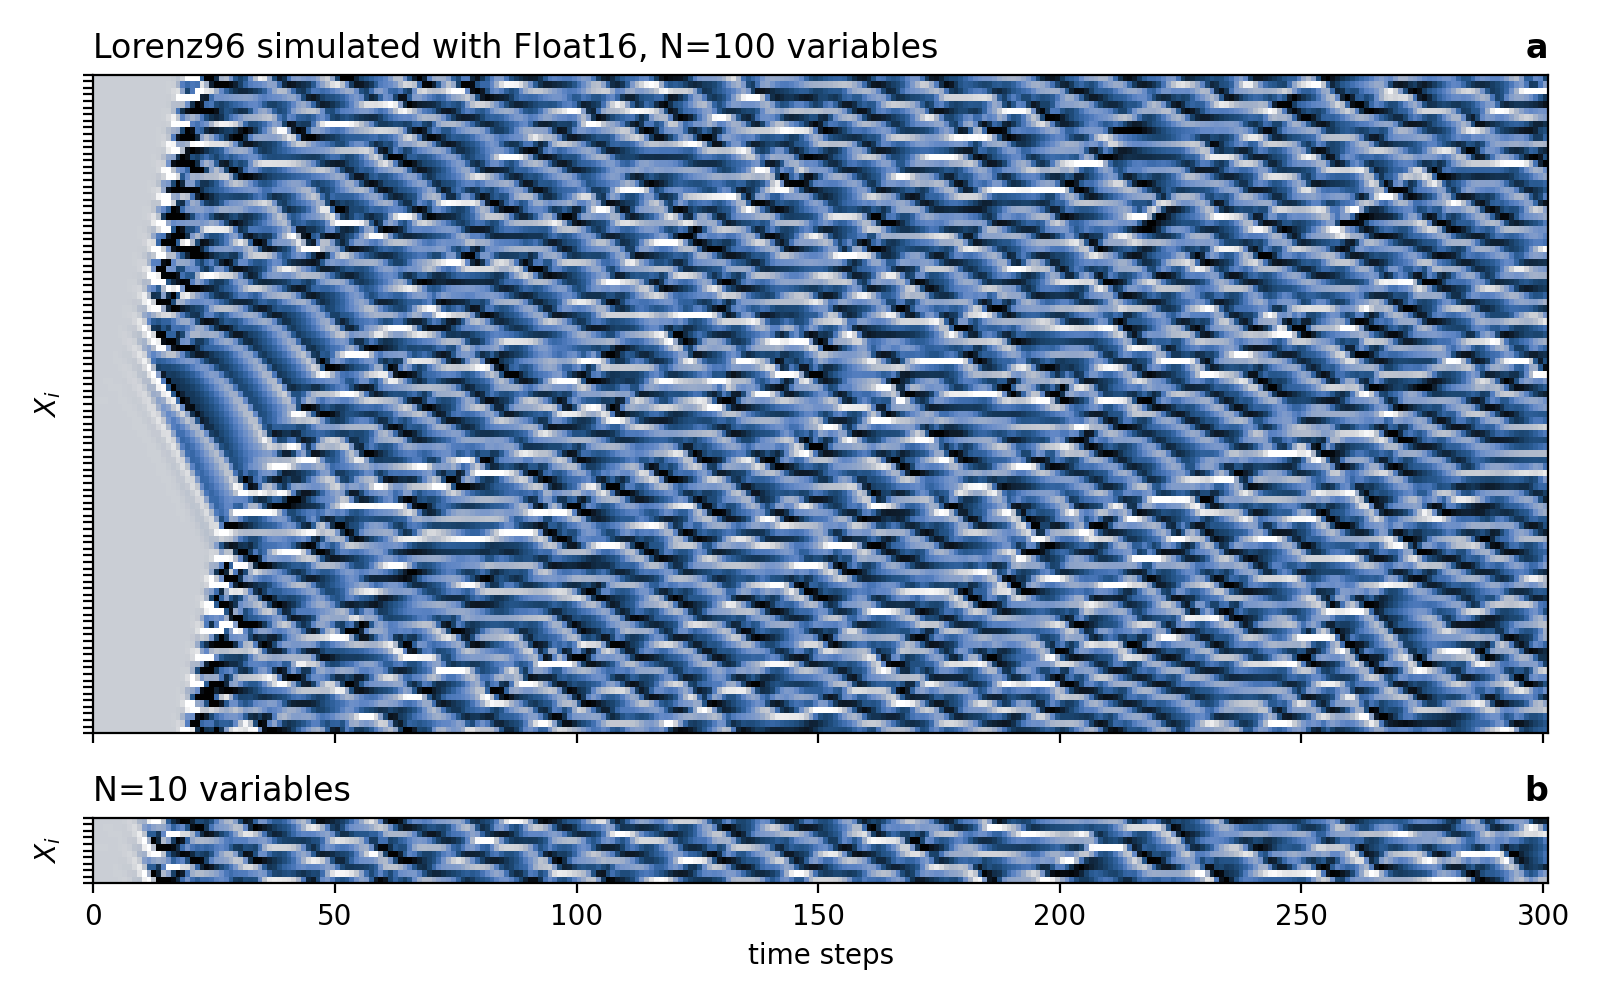
\includegraphics[width=1\textwidth]{Figs/hovmoeller.png}
%\caption{Solution of the Lorenz 1996 model presented as Hovmoeller diagram. (a) Float64 arithmetic, (b) Posit(16,1) arithmetic.}
%\label{fig:L96_hovmoeller}
%\end{figure}

A Hovmoeller diagram illustrates the chaotic dynamics simulated by the Lorenz 1996 model (Fig. \ref{fig:L96_hovmoeller}). The initial perturbation in $X_1$ is advected throughout the domain within the first time steps. After this first wake, the model's state becomes chaotic. Posit(16,1) represents well the dynamic, as shown in the comparison with Float64 for reference.

To quantify the forecast error, we run a set of 1000 forecasts per number format, starting from a random time step of a long control simulation. The simulation with Float64 is taken as reference truth. Float16 has an exponential error growth that starts much earlier than the error growth for Posit(16,1) (Fig. \ref{fig:L96_error}). Both formats have on average an identical error growth rate. Posits clearly cause a reduced rounding error compared to floats at all lead times, making posits a better suited number format for the simulation of the Lorenz 1996 model.

We now use the long control simulation with Float64 to produce a dataset that contains all prognostic variables as well as the arithmetic results of all intermediate terms calculated for the tendencies. 16-bit sonums are trained with this dataset, such that they can self-organize around the numbers that occur most frequently within the Lorenz 1996 model (Fig. \ref{fig:Sonum_decprec}b). Consequently, Sonum16 has a slightly higher decimal precision compared to posits for the mode of the data distribution. A second mode is created for the tendencies, for which numbers of the order of $10^{-1}$ frequently occur. The decimal precision of Sonum16 drastically drops beyond the largest numbers $O(100)$ in the Lorenz 1996 model, as no bitpatterns have to be used to encode these real numbers.

After training, the sonum circle (Fig. \ref{fig:sonum_circle}) is defined. All arithmetic operations are precomputed creating look-up tables for multiplication, addition and subtraction. No look-up table is created for division as the Lorenz 1996 equations (Eq. \ref{eq:L96s}) are written division-free ($s^{-1}$ is precomputed). We can now quantify the forecast error as for floats and posits, running a set of 1000 forecasts from the same initial conditions as used for floats and posits.

Sonum16 has a smaller forecast error compared to posits for the important lead times where the normalised RMSE exceeds 1\% (Fig. \ref{fig:L96_error}). Interestingly, although the error growth is much faster for the first time steps, it levels off afterwards and approaches the same error growth rate as for floats and posits once the normalised RMSE exceeds about 1\%. This points towards a higher potential of Sonum16, when the cause of the initial rapid error growth is understood and circumvented with adjustments in the training method. As discussed in the previous section, sonums can be trained to minimize the average decimal rounding error, an aspect that requires further analysis to understand the optimal distribution of decimal precision for a given application. Nevertheless, sonums already provide perspectives towards an optimal number format for a given application. The main characteristics presumably are: (i) high precision for the most frequently occurring numbers, (ii) a tapered precision towards the smallest numbers and (iii) no redundant bitpatterns for very large and very small numbers that do not occur. Posits fulfill these criteria better than floats, which is likely the reason why they outperform floats in the applications presented here.

%\begin{figure}
%\includegraphics[width=1\textwidth]{Figs/L96_error.pdf}
%\caption{Error growth in the Lorenz 1996 system as simulated with Float16, Posit(16,1) or Sonum16. The error has been normalised by the climatological forecast error. Shaded areas denote the interquartile range of 1000 forecasts with the respective format.}
%\label{fig:L96_error}
%\end{figure}
\end{comment}